\chapter{Pre-calculus results}

This chapter is made to provide a bunch of useful pre-calculus results.

\section{Algebra}
\subsection{Arithmetic Operations}

\[
  a(b + c) = ab + ac \hspace{5em}
  \frac{a + b}b = \frac ab + \frac cb \hspace{5em}
  \frac ab + \frac cd = \frac{ad + bc}{bd} \hspace{5em}
  \frac{\sfrac ab}{\sfrac cd} = \frac ab \times \frac dc = \frac{ad}{bc}
\]

\subsection{Exponents and Radicals}

\[
  x^m x^n = x^{m + n}\hspace{4em}
  (x^m)^n = x^{mn} \hspace{4em}
  (xy)^n = x^n y^n \hspace{4em}
  x^{\sfrac 1n} = \sqrt n \hspace{4em}
  \nthroot n{xy} = \nthroot nx \nthroot ny
\]

\[
  \frac{x^m}{x^n} = x^{m - n} \hspace{4em}
  x^{-1} = \frac 1{x^n} \hspace{4em}
  \parens*{\frac xy}^n = \frac{x^n}{y^n} \hspace{4em}
  x^{\sfrac mn} = \nthroot n{x^m} = \parens*{\nthroot nx}^m \hspace{4em}
  \nthroot n{\frac xy} = \frac{\nthroot nx}{\nthroot xy}
\]

\subsection{Factoring Special Polynomials}
\[
  x^2 - y^2 = (x + y) (x - y) \hspace{5em}
  x^3 + y^3 = (x + y) (x^2 - xy + y^2) \hspace{5em}
  x^3 - y^3 = (x - y) (x^2 + xy + y^2)
\]
\subsection{Binomial Theorem}

\[
  (x + y)^2 = x^2 + 2xy + y^2 \hspace{5em}
  (x - y)^2 = x^2 - 2xy + y^2 \hspace{5em}
\]

\[
  (x + y)^3 = x^3 + 3x^2y + 3xy^2 + y^3 \hspace{5em}
  (x - y)^3 = x^3 - 3x^2y + 3xy^2 - y^3 
\]
In general we have:
\[
  (x + y)^n = x^n + nx^{n-1}y + \frac{n(n-1)}2 x^{n-2}y^2 + \cdots + \binom nk x^{n-k}y^k + \cdots + nxy^{n-1} + y^n
\]

where

\begin{align*}
  \binom nk &= \frac{n!}{k! (n - k)!} \\
            &= \frac{n \cdot (n-1) \cdot (n-2) \cdot (n-3) \cdot \cdots \cdot 3 \cdot 2 \cdot 1}{k!(n - k)!}\\
            &= \frac{n \cdot (n-1) \cdot \cdots \cdot (n - k + 1) \cdot (n-k)!}{k!(n - k)!}\\
            &= \frac{n \cdot (n-1) \cdot \cdots \cdot (n - k + 1)}{k \cdot (k-1) \cdot (k-2) \cdot \cdots \cdot 2 \cdot 1}
\end{align*}

\subsection{Quadratic Formula}
\[
  \text{if } ax^2 + bx + c = 0, \text{ then } x = \frac{b \pm \sqrt{b^2 - 4ac}}{2a}
\]

\subsection{Inequalites and Absolute Value}
\begin{itemize}
  \item If $a < b$ and $b < c$, then $a < c$
  \item If $a < b$, then $a + c < b + c$
  \item If $a < b$ and $c > 0$, then $ac < bc$
  \item If $a < b$ and $c < 0$, then $ac > bc$
  \item If $a > 0$, then
    \begin{itemize}
      \item $\abs*{x} = a \quad$ means $\quad x = a$ or $x = -a$
      \item $\abs*{x} < a \quad$ means $\quad -a < x < a$
      \item $\abs*{x} > a \quad$ means $\quad x > a$ or $x < -a$
    \end{itemize}
\end{itemize}

\section{Geometry}
\subsection{Geometric Formulas}
Formulas for area $A$, circumference $C$, and volume $V$.
\begin{center}
  \begin{tabular}{llllll}
    Triangle & Circle & Sector of Circle & Sphere & Cylinder & Cone\\[0.3cm]
    $A = \frac{1}{2}bh$ & $A = \pi r^2$ & $A = \frac{1}{2}r^2\theta$ & $V = \frac34 \pi r^3$ & $V = \pi r^2 h$ & $V = \frac13 \pi r^2 h$ \\[0.3cm]
    $= \frac{1}{2}ab \sin \theta$ & $C = 2\pi r$ & $s = r\theta$ ($\theta$ in radians) & $A = 4 \pi r^2$ & & $A = \pi r \sqrt{r^2 + h^2}$
  \end{tabular}
\end{center}

\subsection{Distance and Midpoint Formulas}
Distance between $P_1(x_1, y_1)$ and $P_2(x_2, y_2)$.
\[d = \sqrt{(x_2 - x_1)^2 + (y_2 - y_1)^2}\]
Midpoint of $\overline P_1 P_2$.
\[\parens*{\frac{x_1 + x_2}2 , \frac{y_1 + y_2}2}\]

\subsection{Lines}
Slope of line through $P_1(x_1, y_1)$ and $P_2(x_2, y_2)$.
\[m = \frac{y_2 - y_1}{x_2 - x_1}\]
Point-slope equation of line through $P_1(x_1, y_1)$ with slope $m$.
\[y - y_1 = m(x - x_1)\]
Slope-intercept equation of line with slope $m$ and $y$-intercept b.
\[y = mx + b\]

\subsection{Circles}
Equation of the circle with center ($h,k$) and radious $r$.
\[(x - h)^2 + (y-k)^2 = r^2\]

\section{Trigonometry}
\subsection{Angle Measurement}
\[\pi \text{ radians } = 180^{\circ} \qquad 1^{\circ} = \frac{\pi}{180}rad \qquad s = r \theta \quad (\theta \text{ in radians}, s \text{ arc lenght})\]

\subsection{Right Angle Trigonometry}
\[
  \sin \theta = \frac{\text{opp}}{\text{hyp}} \qquad
  \cos \theta = \frac{\text{adj}}{\text{hyp}} \qquad
  \tan \theta = \frac{\text{opp}}{\text{adj}}
\]
\[
  \csc \theta = \frac{\text{hyp}}{\text{opp}} \qquad
  \sec \theta = \frac{\text{hyp}}{\text{adj}} \qquad
  \cot \theta = \frac{\text{adj}}{\text{opp}}
\]

\subsection{Trigonometric Functions}

\[
  \sin \theta = \frac yr \qquad
  \cos \theta = \frac xr \qquad
  \tan \theta = \frac yx
\]
\[
  \sin \theta = \frac ry \qquad
  \cos \theta = \frac rx \qquad
  \tan \theta = \frac xy
\]
  \begin{center}
    \begin{tikzpicture}
      \draw[->] (0,0) -- (5,0) node[right] {$x$};
      \draw[->] (0,0) -- (0,5) node[above] {$y$};
      \draw[green, thick] (0,0) -- (4,4);
      \fill (3,3) circle (2pt) node[right] {$(x,y)$};
      \draw[dashed] (3,0) -- (3,3);
      \draw (0.5,0) arc (0:45:0.5) node[anchor=west] {$\theta$};
      \draw (1.5,1.5) node[right] {$r$};
      \draw (3,0.2) -- (3,0) -- (2.8,0);
    \end{tikzpicture}
  \end{center}

\subsection{Graphs of Trigonometric Functions}

\begin{figure}[h!]
    \centering
    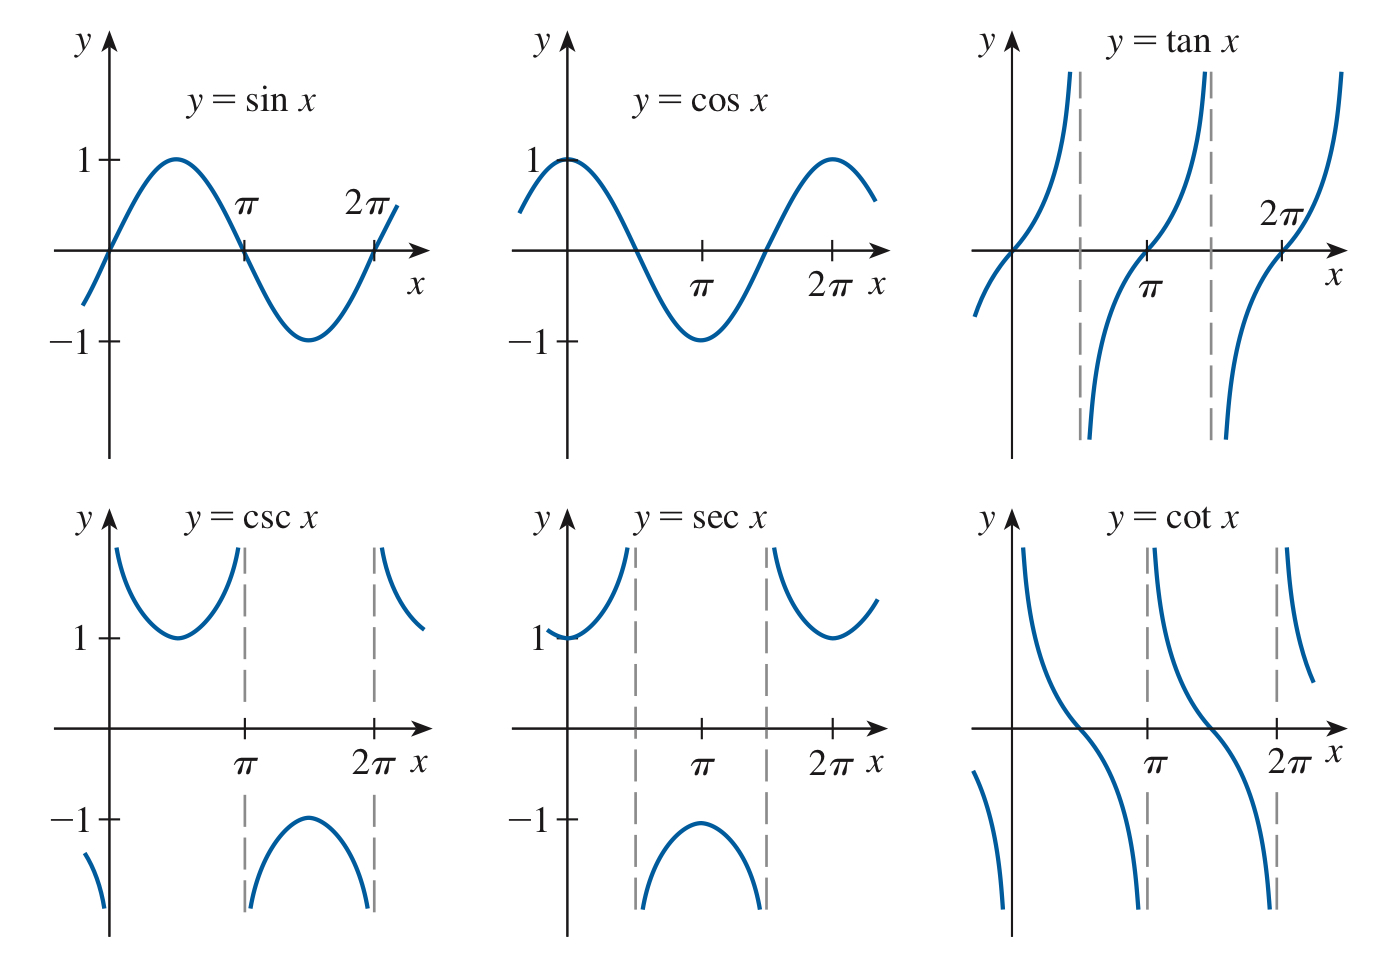
\includegraphics[width=0.6\textwidth]{graphs-trig.jpg}
\end{figure}

\subsection{Trigonometric Functions of Important Angles}

\begin{center}
  \begin{tabular}{llllll}
    $\theta$ & Radians & $\sin \theta$ & $\cos \theta$ & $\tan \theta$\\[0.3cm]
    $0^{\circ}$ & $0$ & 0 & 1 & 0 \\[0.3cm]
    $30^{\circ}$ & $\sfrac{\pi}6$ & $\sfrac12$ & $\sfrac{\sqrt 3}2$ & $\sfrac{\sqrt 3}3$ \\[0.3cm]
    $45^{\circ}$ & $\sfrac{\pi}4$ & $\sfrac{\sqrt 2}2$ & $\sfrac{\sqrt 2}2$ & 1 \\[0.3cm]
    $60^{\circ}$ & $\sfrac{\pi}3$ & $\sfrac{\sqrt 3}2$ & $\sfrac12$ & $\sqrt 3$ \\[0.3cm]
    $90^{\circ}$ & $\sfrac{\pi}2$ & 1 & 0 & - \\[0.3cm]
  \end{tabular}
\end{center}

